\chapter{Methodology}
\label{chap:methodology}

\section{Experimental Setup}
\label{sec:experimental-setup}

[To be completed: overview of simulation environment, agent initialization, scenario design, and logging infrastructure.]

\section{System Design}
\label{sec:system-design}

Our neuro-symbolic planning system extends a re-implementation of the Generative Agents architecture \cite{parkGenerativeAgentsInteractive2023a} with modifications enabling controlled comparison between purely neural planning (baseline) and neuro-symbolic planning (our approach).

\subsection{System Architecture}
\label{subsec:system-architecture}

The implementation transforms the original monolithic Generative Agents codebase into a modular, service-oriented architecture:

\begin{enumerate}
\item \textbf{Repository Layer}: Abstracts external dependencies (LLM APIs, file storage) behind interfaces. \texttt{LLMRepository} supports both OpenAI (production) and mock providers (testing). \texttt{EnvironmentRepository} abstracts world state persistence.

\item \textbf{Service Layer}: Encapsulates cognitive capabilities in swappable interfaces:
\begin{itemize}
\item \texttt{PlanningService}: Daily planning and task decomposition
\item \texttt{DialogueService}: Conversation generation
\item \texttt{PerceptionService}: Environment observation and memory retrieval
\item \texttt{ReflectionService}: Memory summarization
\item \texttt{EnvironmentService}: Spatial navigation and object interaction
\end{itemize}

\item \textbf{Orchestration Layer}: The simulation loop consumes services through interfaces, configured via environment variables (\texttt{LLM\_PROVIDER}, \texttt{PLAN\_MODULE}) controlling which implementations run.
\end{enumerate}

\textbf{Key Design Principle}: The \texttt{PlanningService} abstraction enables side-by-side comparison of baseline (LLM-only hierarchical planning) and neuro-symbolic planning by ensuring both share identical environment state, memory retrieval, and LLM infrastructure. Only the planning logic differs, isolating the independent variable.

\begin{figure}[H]
\centering
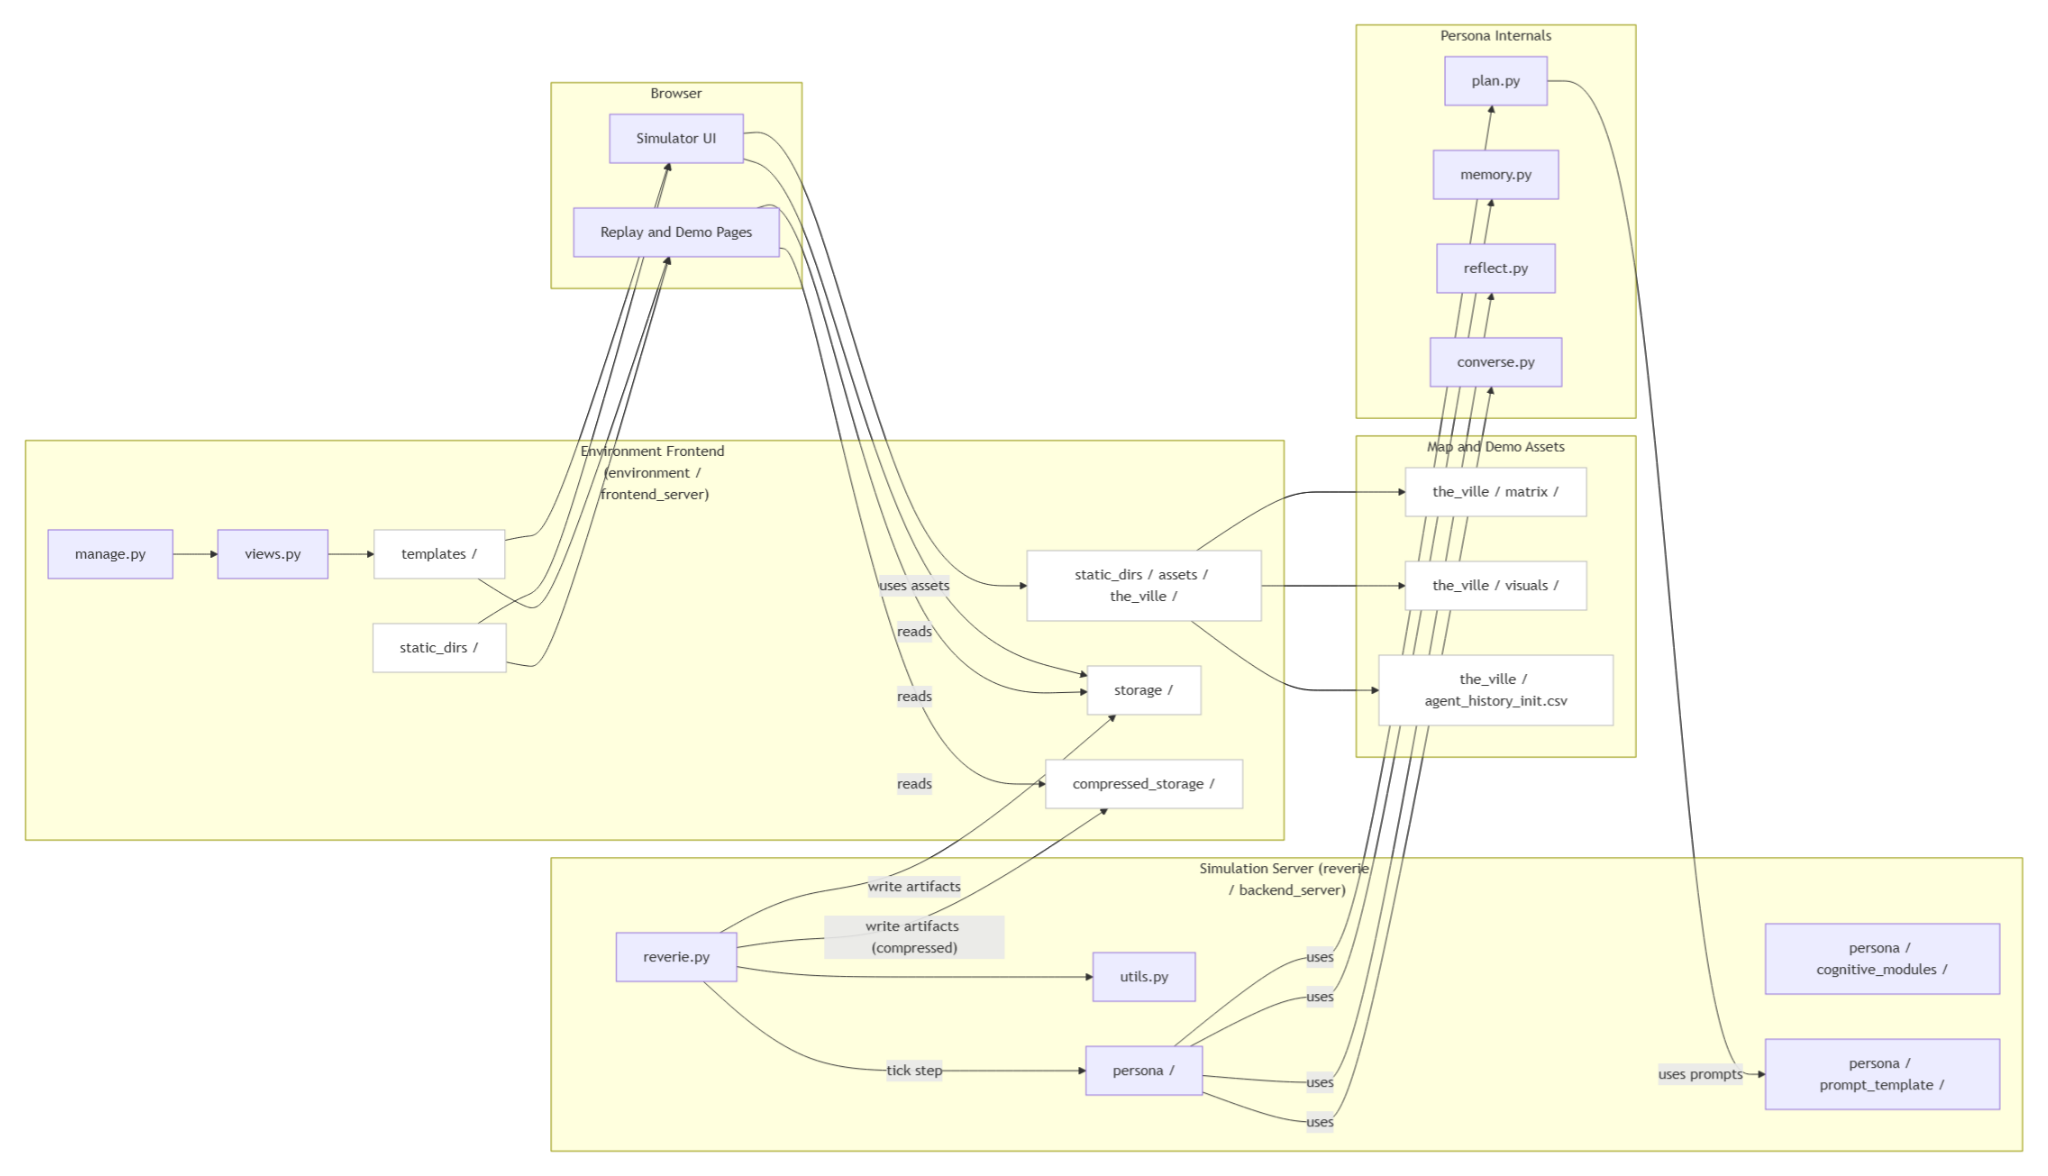
\includegraphics[width=\textwidth]{Pictures/Code Structure - before.png}
\caption{Original monolithic architecture from the Generative Agents codebase \cite{parkGenerativeAgentsInteractive2023a}, showing tightly coupled components without clear separation of concerns.}
\label{fig:code-structure-architecture-before}
\end{figure}

\subsection{Neuro-Symbolic Planning Pipeline}
\label{subsec:neuro-symbolic-pipeline}
\textbf{[section is subject to changes after final implementation]}

\begin{figure}[H]
\centering
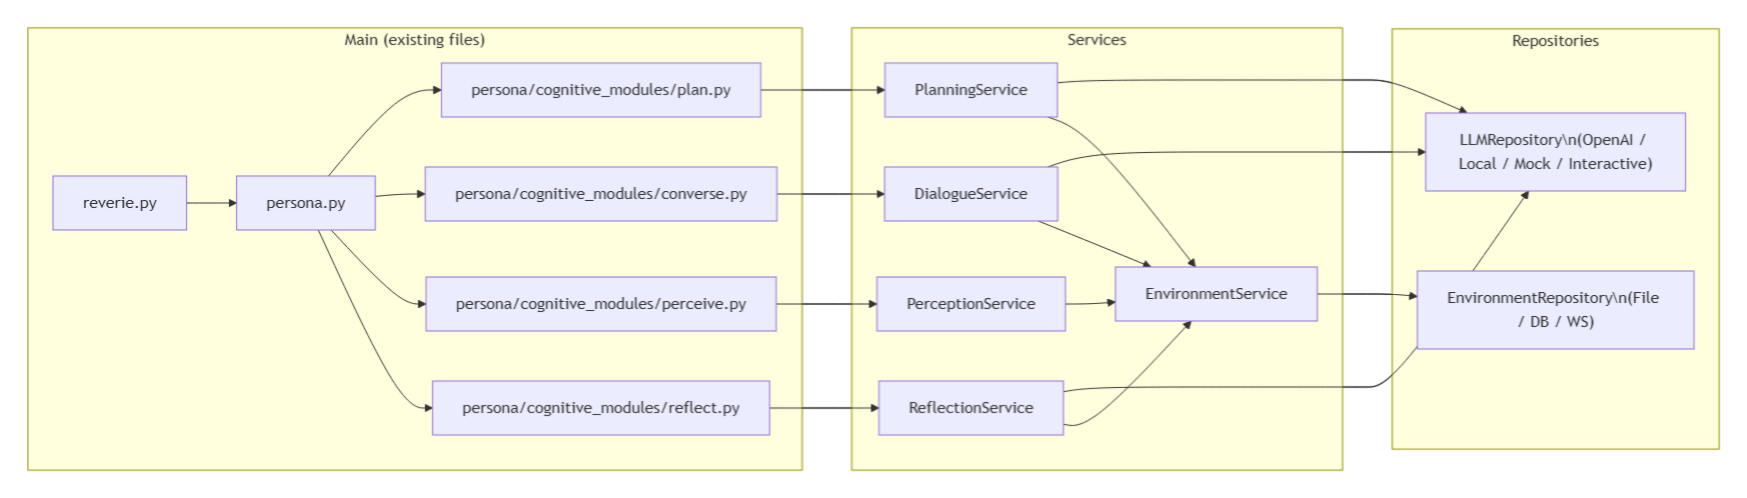
\includegraphics[width=\textwidth]{Pictures/Code Structure - after.png}
\caption{Refactored service-oriented architecture with Repository, Service, and Orchestration layers. The \texttt{PlanningService} abstraction enables controlled comparison between baseline and neuro-symbolic planning implementations.}
\label{fig:code-structure-architecture-after}
\end{figure}

We implement a three-stage LLM-propose/symbolic-validate framework \cite{kambhampatiLLMsCantPlan2024,tantakounLLMsPlanningModelers2025,huangPlanningDarkLLMSymbolic2024}:

\begin{enumerate}
\item \textbf{Task Generation}: The LLM generates daily tasks from memory, grounding them in wants, needs, and commitments \cite{parkGenerativeAgentsInteractive2023a}.

\item \textbf{Action Decomposition}: Tasks decompose into atomic actions with environment parameters. Example: ``complete assignment'' $\rightarrow$ \texttt{open-laptop}, \texttt{navigate-to-file}, \texttt{work-on-document(90min)}, \texttt{submit-via-portal}.

\item \textbf{Schema Generation \& Validation}: The LLM generates PDDL schemas (preconditions, effects, durations) for each action. A symbolic validator checks causal consistency, temporal feasibility, resource limits, and environmental invariants. Violations trigger diagnostic feedback (e.g., ``unsatisfied precondition \texttt{(at-location student hall)}'') for iterative LLM repair until constraints satisfy or iteration budget exhausts.
\end{enumerate}

\section{Quantitative Evaluation: Constraint Violation Analysis}
\label{sec:quantitative-evaluation}

[To be completed: automated evaluation comparing the hierarchical planning baseline against our validator-augmented system. The validator will automatically detect and flag constraint violations such as attempting to use items that are not available, scheduling overlapping activities, violating location constraints, or executing actions whose preconditions are not satisfied. Metrics will include violation counts at day-level and action-level, violation rates per 100 actions, and success rates after optional validator-guided repair rounds.]

\section{User Study: Believability Evaluation}
\label{sec:user-study-believability}

This section describes the human-subjects study testing whether our approach improves perceived believability of agent behavior compared to the baseline Generative Agents architecture \cite{parkGenerativeAgentsInteractive2023a}. We focus on believability of \emph{actions} rather than only personalities or conversations.

\subsection{Objectives and Hypotheses}
\label{subsec:objectives-hypotheses}

Two primary hypotheses:

\begin{itemize}
\item \textbf{H1 (overall believability)}: Participants judge agents powered by our method as more believable overall than the baseline in matched scenarios.
\item \textbf{H2 (action believability)}: For the same scenario, participants flag fewer actions as ``unbelievable'' in our method than in the baseline.
\end{itemize}

Secondary outcomes: (i) perceived causal coherence when the high-level plan is visible, and (ii) free-text reasons participants provide when deeming actions unbelievable (used for qualitative error analysis) \cite{batesRoleEmotionBelievable1994,bogdanovychWhatMakesVirtual2016,tenceAutomatableEvaluationMethod2010,xiaoHowFarAre2024}.

\subsection{Conditions}
\label{subsec:conditions}

Two within-subject conditions on the same simulated world and character seeds:

\begin{enumerate}
\item \textbf{Baseline (GA)}: Faithful re-implementation of Generative Agents \cite{parkGenerativeAgentsInteractive2023a}.
\item \textbf{Ours (Neuro-symbolic)}: Proposed system with symbolic planning and consistency checks integrated into deliberation and action selection.
\end{enumerate}

Each participant evaluates both conditions on the same character and scenario to enable within-subject comparison. Order is counterbalanced (Latin square design) to reduce presentation effects.

\subsection{Participants}
\label{subsec:participants}

Target 10 to 15 adult participants recruited from the university community and online platforms. Inclusion criteria: English proficiency. We run an initial pilot (3 to 4 participants) to validate timing and interface, then proceed to the main study. All participants provide informed consent and can withdraw anytime without penalty.

\subsection{Materials and Stimuli}
\label{subsec:materials-stimuli}

The stimulus for each condition is a replay of a single random character's day. To focus on action believability, we present:

\begin{itemize}
\item time-lapse \emph{video replay} of the agent acting in the world (controllable playback speed, pause/seek);
\item optional overlay with \emph{high-level plan} (intentions and sub-goals) and \emph{low-level action log}; and
\item UI controls to mark an action as unbelievable (``thumbs down''), provide a short reason, and continue.
\end{itemize}

Replays cover the same scenario (e.g., two simulated in-game days) and use the same character profile and randomness seed across conditions, so any variation is attributable to agent architecture (baseline vs. ours) rather than scenario noise.

\subsection{Procedure}
\label{subsec:procedure}

Each session (approximately 30 minutes):

\begin{enumerate}
\item \textbf{Introduction.} Scripted briefing introduces the task and believability as coherence, plausibility, and consistency within world rules \cite{bogdanovychWhatMakesVirtual2016}.
\item \textbf{Practice.} Participants complete a 2 to 3 minute tutorial on the interface using a neutral example not used in the main study.
\item \textbf{Condition A.} Watch the replay, freely scrub, and mark unbelievable actions. For each mark, add a short explanation (optional but encouraged).
\item \textbf{Condition B.} Repeat with the other planner. Order varies across participants; assignment is double-blind.
\item \textbf{Summary ratings.} For each condition: (i) overall believability rating (7-point Likert), (ii) perceived causal coherence rating (7-point Likert), and (iii) preference judgment (forced-choice which was more believable and why).
\end{enumerate}

We record duration until finished and whether the plan overlay was opened, to analyze how explanations affect believability judgments.

\subsection{Measures}
\label{subsec:measures}

We operationalize believability with participant-reported and behavior-linked measures. Higher values indicate higher believability unless noted.

\subsubsection{Primary Outcomes}
\label{subsubsec:primary-outcomes}

\begin{enumerate}
\item \textbf{Overall believability (Likert).} Single item per condition on a 7-point scale: 1 ``not at all believable'', 4 ``moderately believable'', 7 ``extremely believable''. Prompt: ``How believable was the agent's behaviour overall in this replay?''

\item \textbf{Action-level unbelievable rate (event-normalized).} Participants flag any action as unbelievable. Let $F$ be flagged action events and $A$ be \emph{atomic actions} viewed (from action log restricted to watched timestamps). The rate is
\begin{equation}
r_{\mathrm{unbel}} = \frac{F}{A} \times 100\,,
\end{equation}
expressed as flags per 100 atomic actions. Multiple flags within 2 seconds around the same atomic action merge into one.

\item \textbf{Pairwise preference.} Forced-choice: ``Which replay was more believable overall?'' (Baseline vs. Ours).
\end{enumerate}

\subsubsection{Secondary Outcomes}
\label{subsubsec:secondary-outcomes}

\begin{itemize}
\item \textbf{Causal coherence (Likert).} 7-point rating: 1 ``not coherent'', 7 ``highly coherent''.
\item \textbf{Plan adherence (Likert).} 7-point rating of alignment between visible high-level plan and observed actions.
\item \textbf{Unbelievable-action categories (coded).} Free-text reasons are open-coded into categories: goal inconsistency, environment rule violation, temporal implausibility, social norm violation, low-level control failure. Two independent coders label a stratified sample ($\geq 30\%$ of flags); disagreements are adjudicated and inter-rater agreement (Cohen's $\kappa$) is reported.
\end{itemize}

\textbf{Logged covariates (for analysis, not outcomes):} condition order, scenario ID, participant playback time, number of overlay openings, and self-reported prior experience with simulations/games. These are used as covariates in exploratory models and to check for order effects.

\subsection{Data Quality and Exclusion}
\label{subsec:data-quality}

Sessions are excluded if participants fail an attention check (simple comprehension question about the replay), leave more than half the session unanswered, or complete in less than one-third of median time. We pre-register exclusion rules prior to data collection.

\subsection{Analysis}
\label{subsec:analysis}

We analyze overall believability with within-subject comparisons (paired $t$-test when normality holds; otherwise Wilcoxon signed-rank). For action-level data, we fit a mixed-effects logistic regression on the probability that an action is flagged:

\begin{verbatim}
flag ~ condition + (1|participant) + (1|scenario)
\end{verbatim}

We report effect sizes (Cohen's $d$ or odds ratios) and 95\% CIs. Qualitative reasons are open-coded into failure categories (goal inconsistency, environment rule violation) to contextualize quantitative effects.

\subsection{Ethics}
\label{subsec:ethics}

The study involves minimal risk. No personal data beyond demographics is collected; all logs are anonymized and stored on encrypted drives.

\subsection{Power and Timing}
\label{subsec:power-timing}

A conservative power analysis for within-subject design with moderate effect (Cohen's $d=0.5$, $\alpha=0.05$, power $=0.8$) suggests $N\approx 34$. Given resource constraints, we aim for 10 to 15 valid participants after exclusions; the pilot is analyzed descriptively and may inform small interface adjustments.
